%
\section{Results \& Discussion}\label{sec:Results & Discussion}
%
In this chapter, I summarize the results obtained from my experiments. My experiment is mainly focused on automating the open-source software discovery and finding the suitable vulnerability database for vulnerability analysis.

\subsection{Open-Source Software Discovery}
As defined previously, the scanner has to scan \acs{OSS} components from different application framework projects. This means that the scanner should have function which as to give a common output even if it scans different project. In this experiment, first I have tried using manual scrapping to understand how the \acs{OSS} components can be identified and where it is registered inside the project. The manual scrapping will be an easy solution if it is a small project but it will be a time consuming process if it is performed in a large scale project. Figure ~\ref{fig:laravel}, ~\ref{fig:ruby}, ~\ref{fig:gradle}, ~\ref{fig:django}, ~\ref{fig:pom} and ~\ref{fig:dotnet} shows where exactly the OSS components are registered in the project. From these files with the help of manual scrapping, we can extract the component name and version by traditional copy \& pasting technique. Then we have to search vulnerability information of each component in the vulnerability database. Therefore manual scrapping for big projects will be time consuming task and also there is possibility for human errors.
\begin{figure}[h!]
	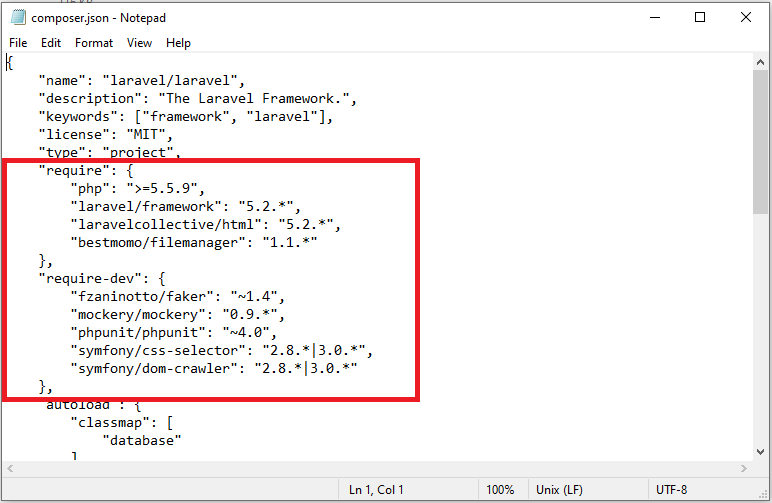
\includegraphics[width=15cm]{includes/laravel.PNG}
	\centering
	\caption{Laravel project config file}
	\label{fig:laravel}
\end{figure}
\begin{figure}[H]
	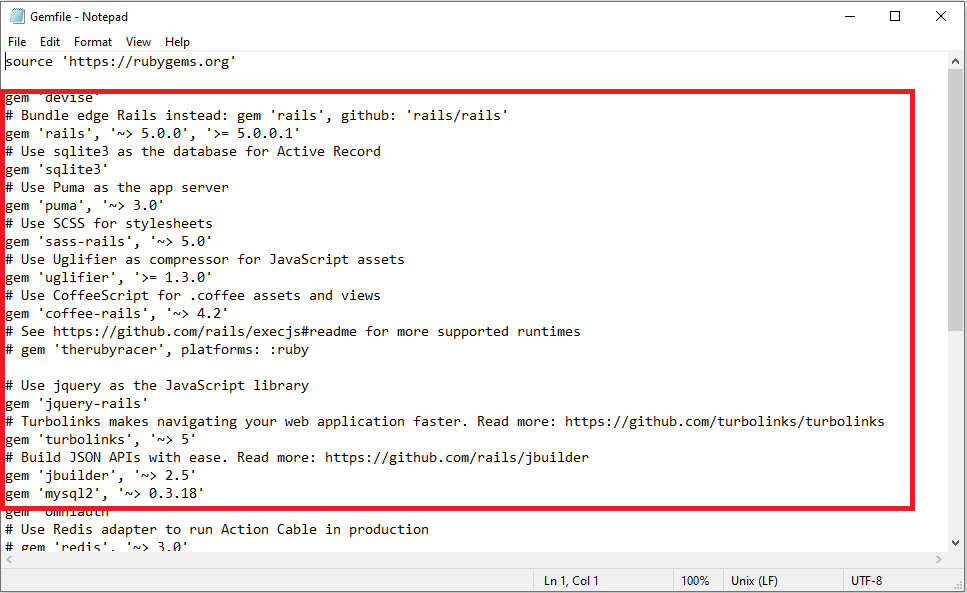
\includegraphics[width=15cm]{includes/ruby.PNG}
	\centering
	\caption{Ruby on Rails project config file}
	\label{fig:ruby}
\end{figure}
\begin{figure}[H]
	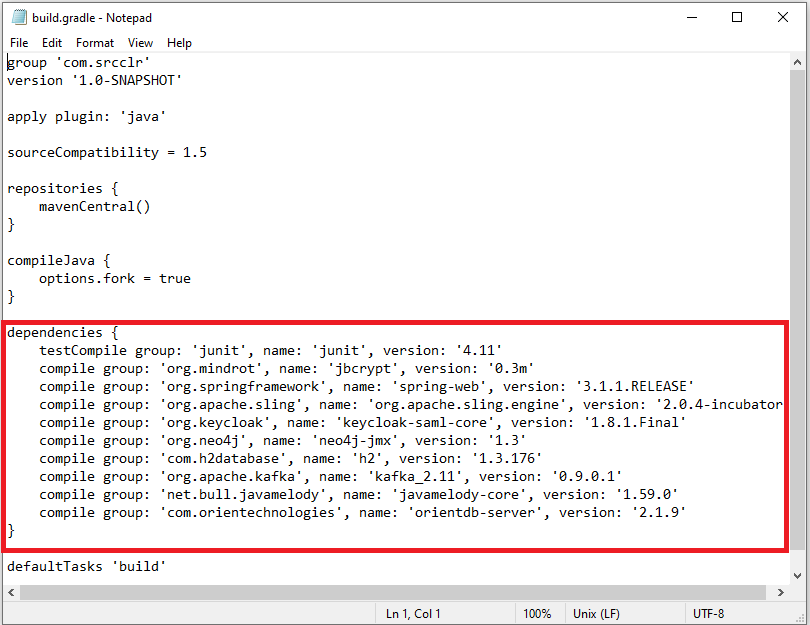
\includegraphics[width=15cm]{includes/gradle.PNG}
	\centering
	\caption{Gradle project config file}
	\label{fig:gradle}
\end{figure}
\begin{figure}[H]
	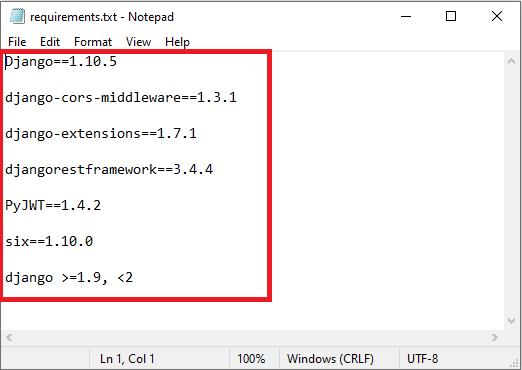
\includegraphics[width=15cm]{includes/django.PNG}
	\centering
	\caption{Django project config file}
	\label{fig:django}
\end{figure}
\begin{figure}[H]
	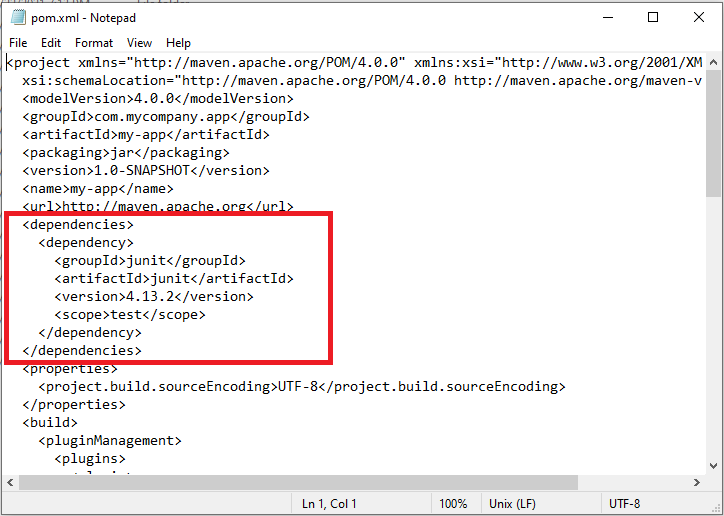
\includegraphics[width=15cm]{includes/pom.PNG}
	\centering
	\caption{Maven project config file}
	\label{fig:pom}
\end{figure}
\begin{figure}[H]
	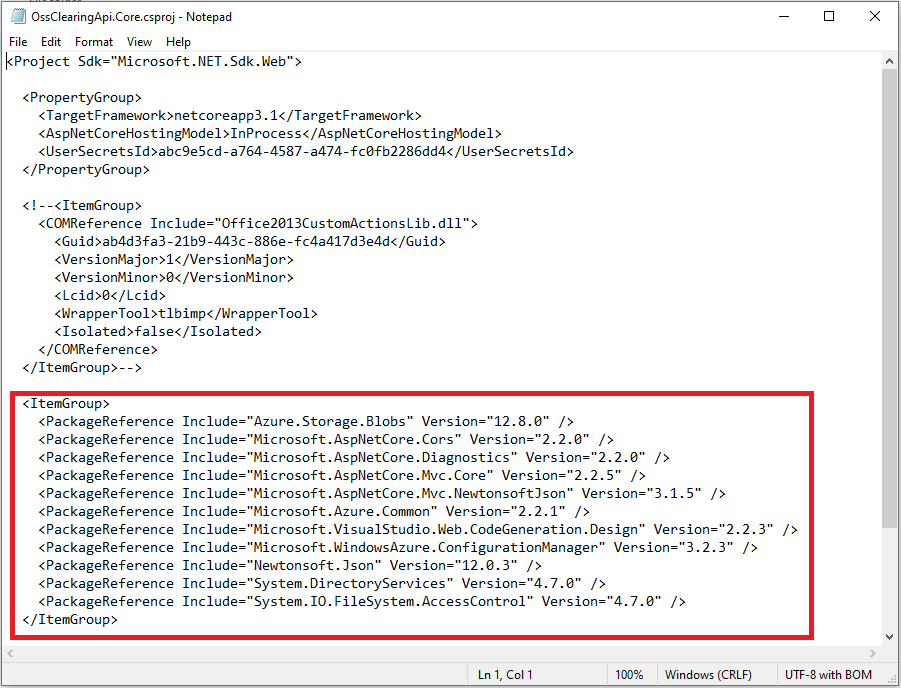
\includegraphics[width=15cm]{includes/dotnet.PNG}
	\centering
	\caption{Dotnet project config file}
	\label{fig:dotnet}
\end{figure}

\paragraph{}
After experimenting the manual scraping, I tried automating the process by using Automated scraping methods. DOM parsing and text pattern matching methods are used for automated extraction. The main reason to use these two scraping methods is that the scanning takes place in client side. These two methods os scrapping can be achieved by using Angular framework. For projects like Dotnet, Gradle, Laravel and Maven DOM parsing method is used because the config files of these projects are XML and JSON files. The text pattern matching methods are used for Django and Ruby on Rails projects. Finally by using these two scraping method a generic function is created to give a final output as a JSON object. Figure ~\ref{fig:clientOutput} will illustrate the extracted component from Ruby on Rails project within the browser. Along with the component name and version I have also showed from which file it is extracted. 
\newpage
\begin{figure}[H]
	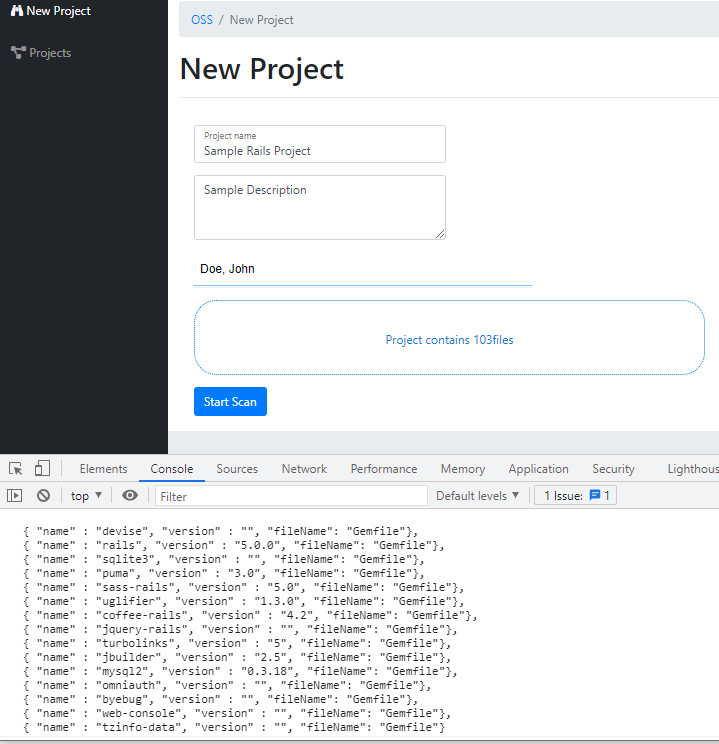
\includegraphics[width=15cm]{includes/clientOutput.PNG}
	\centering
	\caption{OSS component name and version extraction from Ruby on Rails project}
	\label{fig:clientOutput}
\end{figure}

\subsection{Vulnerability Databases}
Once 
